% arara: pdflatex: { shell: true, draft: true }
% arara: makeglossaries
% arara: biber
% arara: pdflatex: { shell: true, synctex: true }
% arara: pdflatex: { shell: true, synctex: true }

\documentclass[12pt,DIV14,BCOR10mm,a4paper,parskip=half-,headsepline,headinclude,english,ngerman,bibliography=totocnumbered]{scrreprt}

\usepackage{hshhelper_base}

\usepackage{enumitem}

\lstset
{ %Formatting for code in appendix
    numbers=left,
}

%%%%%%%%%%%%%%%%%%%%%%%%%%%%%%%%%%%%%%%%%%%%%%%%%%%%%%%%%%%%%%%%%%%%%%%%%%
\begin{document}    % hier gehts los
  \thispagestyle{empty} % Titelseite

\includegraphics[width=0.2\textwidth]{Wortmarke_WI_schwarz}

   {  ~ \sffamily
  \vfill
  {\Huge\bfseries Sicherheitsuntersuchungsbericht: Applikation \enquote{HsH-Helper} der Gruppe B}
  \bigskip

  {\Large
  Dennis Grabowski, Julius Zint, Philip Matesanz, Torben Voltmer \\[2ex]
  Masterprojekt \enquote{Entwicklung und Analyse einer sicheren \\Web-Anwendung} \\
  Wintersemester 18/19
 \\[5ex]
   \today }
}
 \vfill

  ~ \hfill
  
\includegraphics[height=0.3\paperheight]{H_WI_Pantone1665}

\vspace*{-3cm}

\tableofcontents  % Inhaltsverzeichnis

\chapter{Ausgelieferte virtuelle Maschine ist nicht benutzbar}

Innerhalb der VM können die Aktionen \enquote{Nutzer anlegen} sowie \enquote{Datei hochladen} nicht verwendet werden, da beide bei normaler, erwarteter Nutzung zu einem Fehler führen, wie in Anhang \ref{createuser_fail_1} sowie \ref{upload_fail_1} zu sehen ist.
Da wir bereits wussten, dass der seperat ausgelieferte Quellcode funktioniert, waren wir dementsprechend schockiert. 
Diese Fehler bestehen auch, wenn man den Quellcode aus der VM extrahiert und auf seinem Hostrechner via \texttt{sbt run} oder IntelliJ startet.
Komischerweise hat ein \texttt{git diff} bewiesen, dass kein Unterschied zwischen den beiden vorliegenden Quellen besteht.

Aus Interesse haben wir daher versucht, die Ursache des Fehlers herauszufinden, konnten den Ursprung allerdings nicht finden.
Ein Symptom ist zumindest, dass bestimmte Felder nicht korrekt aus dem HTML-Formular gelesen werden konnten.
Beim Anlegen eines neuen Nutzers ist während des Debuggings zumindest das Feld \enquote{username} in dem \texttt{AddUserForm}-Objekt leer, obwohl es im \texttt{Form<AddUserForm>}-Objekt noch vorhanden ist.
Wir schätzen, dass das Problem auf nicht vorhandene Getter/Setter der selbst geschriebenen Form-Klassen zurückzuführen ist, da diese nicht ausgeführt werden konnten, als wir diese durch die Funktion \enquote{Execute Code} während des Debuggings ausführen wollten.
Ein weiteres Indiz für diese Annahme ist, dass genau die Getter/Setter des jeweils fehlendem Feld nicht vorhanden sind.
Desweiteren sind die SBT Versionen gleich, Quellcode-Unterschiede bestehen wie bereits beschrieben nicht und der Fehler tritt innerhalb und ausserhalb der VM auf, sofern man den Quellcode aus der VM nimmt.

Es ist möglich, dass weitere Aktionen innerhalb der VM nicht funktionieren. Wir hatten nach diesen 2 Aktionen aufgehört, da sie essentiell wichtige Funktionen für den HsH-Helper sind.
Die hier gefundenen Fehler beziehen sich daher auf den seperat mitgelieferten Quellcode, da dieser nicht unter dieser Problematik leidet.

Es stellte sich später heraus, dass die Probleme durch Löschen des mit ausgeliefertem \texttt{target} Ordners im Hauptverzeichnis des Projekts behoben werden können. Beim vergleichen der VM Version mit der Sourcecode Version mittels \texttt{git diff} sind die Unterscheide im \texttt{target} Ordner nicht aufgefallen, da dieser in der \texttt{.gitignore} Datei eingetragen war.


\chapter{Eingesetzte Methoden und Werkzeuge}

Ein Großteil der Fehler und Sicherheitslücken konnten nur durch die Verwendung eines Browsers und die darin enthaltenen Entwicklerfunktionalitäten gefunden werden. Als Browser wurde Google Chrome und Mozilla Firefox verwendet. Um fehlende Funktionen, wie beispielsweise das Ändern der Quota eines Benutzers, dennoch verwenden zu können, wurden Datenbankeinträge direkt mit dem H2-Browser manipuliert.

Um etwas weniger offensichtliche Sicherheitslücken wie beispielsweise Race Conditions aufzudecken wurden Bash-Skripte verwendet, die das Kommandozeilenwerkzeug \textit{cURL} bedienen, um HTTP-Requests an den Server zu senden. Für eine weitere Race Conditions wurde das Python Programm \textit{race-condition-exploit} \footnote{\url{https://github.com/andresriancho/race-condition-exploit}} verwendet. Um HTTP-Requests zu erstellen und abzusenden wurde die Python-Bibliothek \textit{Requests} \footnote{\url{https://github.com/requests/requests}} verwendet.

Der Webproxy \textit{ZAP} \footnote{\url{https://www.owasp.org/index.php/OWASP_Zed_Attack_Proxy_Project}} kam zum Einsatz, um die HTTP-Requests zu betrachten und zu analysieren. Bei der Suche nach Sicherheitslücken wurden POST-Requests mithilfe des Webproxies manipuliert.

Zur Quelltextinspektion und Debugging kam, wie auch schon in der Enwicklungsphase, IntelliJ IDEA zum Einsatz.

Um möglichst viele Sicherheitslücken (und funktionale Fehler) zu finden, haben wir mehrere Methoden verwendet:

\begin{itemize}
  \item Quelltextinspektion, um generell mit dem Code vertraut zu werden,
  \item Reviews, um spezifische Konzepte genauer zu analysieren,
  \item Szenarios, um potentielle Sicherheitslücken zu definieren,
  \item Penetrationtesting, um für potentielle Schwachstellen Angriffe zu finden und,
  \item zu guter letzt das explorative Testen, in der Hoffnung, doch noch etwas zu finden, was wir bisher übersehen haben.
\end{itemize}

\chapter{Funktionale Fehler}


\section{Dateien und Quota}

\begin{enumerate}
\item Beim Anlegen eines Benutzers kann der Administrator nicht wie gefordert das Speicherplatzlimit angeben.\newline
\textit{+ Betroffene Anforderungen: 6.1}

\item Das Speicherplatzlimit kann niemals angepasst werden, da Änderungen an dem Java-Userobjekt nicht in die Datenbank übertragen werden. Man hat vergessen, die \texttt{save()} Methode auf dem entsprechenden Userobjekt aufzurufen.
\textit{+ Betroffene Anforderungen: 6.3}

\item Beim Anlegen eines Benutzers wird ein fest definiertes Speicherplatzlimit von \enquote{1073741824} verwendet. Dieser Wert wurde offensichtlich in der Annahme getroffen, dass in der Anwendung in Bytes gerechnet wird und würde so ca. einem Gigabyte entsprechen. Tatsächlich rechnet die Anwendung die Bytes einer hochgeladenen Datei in Megabyte um und verwendet die Megabyte-Darstellung in Verbindung mit dem nicht konvertierten Speicherplatzlimit. So entspricht das fest definierte Speicherplatzlimit einem faktischen Limit von einem PB. Im Ergebnis führt die Umsetzung in Verbindung mit dem gewählten Standardlimit dazu, dass es realistisch nie erreicht werden wird. Es ist so gänzlich wirkungslos.\newline
\textit{+ Betroffene Anforderungen: 6.1, 6.3}

\item Die Umrechnung von Byte in Megabyte rundet auf. Dies führt dazu, dass eine Datei die kleiner als ein Megabyte ist trotzdem ein Megabyte von der Quota beansprucht.\newline
\textit{+ Betroffene Anforderungen: Keine}

\item Beim Überschreiben einer Datei durch einen anderen Nutzer wird der Speicherplatzverbrauch falsch kalkuliert. Der Nutzer, der die Datei überschrieben hat, bekommmt die Differenz gutgeschrieben, während beim originale Besitzer der Datei keine Änderungen am Speicherplatzverbrauch vorgenommen werden. Dadurch kann ein Benutzer sein Speicherplatz-Limit erhöhen: Er muss nur Dateien von anderen Benutzer auf die er schreibberechtigung hat mit kleineren Dateien überschreiben. Wäre die Quota eines Dateibesitzers theoretisch überschritten, könnte die Datei so dennoch überschrieben werden.\newline
\textit{+ Betroffene Anforderungen: 6.3}

\item Die Anwendung extrahiert aus dem Dateinahmen der tatsächlich ausgewählten Datei die Endung. Diese wird dem vom Nutzer angegebenen Dateinamen hinzugefügt und unterliegt keiner expliziten  Längenbeschränkung, diese wird nur in Bezug auf den vom Nutzer explizit angegebenen Namen erzwungen.\newline
\textit{+ Betroffene Anforderungen: Keine}


\item Es ist Benutzern problemlos möglich, mehrere Dateien mit dem gleichen Namen hinzuzufügen. Der für den Upload zuständige Controller-Code erhält vom Anwender einen expliziten Dateinamen (A) und den Namen der ausgewählten Datei (B). Die Anwendung prüft nun, ob der Nutzer bereits eine Datei besitzt, dessen Name A entspricht. Ist dies nicht der Fall, wird die Dateiendung aus B extrahiert und eine Datei erzeugt, die einen zusammengesetzten Namen besitzt: A + \enquote{.} + extension(B).
Wiederholt man den Upload, prüft die Anwendung erneut, ob der Benutzer eine Datei mit dem Namen A hat - was natürlich nicht der Fall ist, denn der endgültige Name der Datei entspricht nicht A.
Die Dateianzeige lässt den Eindruck entstehen, es würde nur eine Datei zu jedem Namen existieren. Dies ist der Verwendung einer TreeMap geschuldet: Die Anwendung lädt alle Dateien, die zum Benutzer gehören und speichert diese als Key in der TreeMap. Die TreeMap stellt die Eindeutigkeit der Keys über die compareTo Methode der entsprechenden Keys bzw. Files sicher. Diese wurde von der anderen Gruppe überschrieben und beinhaltet für den Vergleich lediglich den Dateinamen und den Owner. D.h. wenn man 10 Dateien mit dem gleichen Namen erzeugt, befindet sich in der Treemap nur eine Datei und nur diese wird so angezeigt. Wird die Datei gelöscht, wird die vorherige angezeigt.\newline
\textit{+ Betroffene Anforderungen: 3.3.1}

\item Beim Hochladen von Dateien können die Berechtigungen nicht unmittelbar vergeben werden, dies sollte in einem Request erfolgen.\newline
\textit{+ Betroffene Anforderungen: 3.3.2}
  \end{enumerate}



\section{Gruppen}
\begin{enumerate}[resume]
\item Die Admin-Gruppe ist löschbar, wodurch die Applikation effektiv unbenutzbar wird. Es gibt zwar eigentlich eine Prüfung, ob versucht wird die Admin-Gruppe zu löschen, diese kann aber einfach umgangen werden. Trägt man im Gruppe-Löschen Formular eine Variation des Gruppennamens ein, die nicht exakt \enquote{admin} entspricht (wie zum Beipiel \enquote{aDmin}, wird die Gruppe gelöscht\footnote{Siehe die Funktion \texttt{isDeletableGroup} in \texttt{GroupManagerService}}. Da bei Aufruf jeder Seite die Gruppe geladen wird, funktioniert nach dem Löschen der Gruppe keine Seite mehr. Es gibt eine NullPointerException in der \texttt{isAdmin} Methode in \texttt{Authorization}.\newline
\textit{+ Betroffene Anforderungen: 5.8}

\item Die Alle-Gruppe ist analog zur Admin-Gruppe löschbar. Nach dem Löschen dieser Gruppe funktioniert allerdings weiterhin vereinzelt Funktionalität.\newline
\textit{+ Betroffene Anforderungen: 5.8}

\item Gruppen, für die Dateiberechtigungen angelegt wurden, können nicht vollständig gelöscht werden. Im Code werden manuell Owner der Gruppe und Mitglieder der Gruppe gelöscht. Zu diesem Zeitpunkt ist die Gruppe \enquote{halb} gelöscht. Der anschließende \texttt{delete} Aufruf schlägt aber fehl, da Integriätsbedingungen in der Datenbank durch das löschen verletzt werden würden. Es wird eine Exception geworfen. In der Folge befindet sich die Datenbank in einem inkonsistenten Zustand. Die Gruppe wird dem Admin noch angezeigt, aber sie ist nichtmehr aufrufbar.\newline
\textit{+ Betroffene Anforderungen: 5.4}

\end{enumerate}

\section{Single Sign On}
\begin{enumerate}[resume]
 \item Der Single Sign On ist hart codiert für die zwei in den Anforderungen gestellten Testfälle. Andere Webdienste können so nicht hinzugefügt werden. Die Oberfläche bietet die Möglichkeit Namen für Benutzer- und Passwort-Parameter zu hinterlegen, diese werden allerdings nicht verwendet.\newline
\textit{+ Betroffene Anforderungen: 2.1, 2.2}
  
\item Die Anwendung prüft, ob in der angegebenen URL für den Webservice die entsprechenden Hostnames von ICMS und Bibliothek enthalten sind. Ist dies nicht der Fall kann der Webservice zwar angelegt werden und Nutzer können Zugangsdaten hinterlegen, der tatsächliche Single Sign On führt dann jedoch zu einer Exception. Bei der vorliegenden Anwendung handelt es sich um eine Debug Version, die zu der Exception noch Code-Ausschnitte anzeigt. Nutzer, eingeschlossen Administratoren, sollten niemals Java Exceptions einsehen können.\newline
\textit{+ Betroffene Anforderungen: 2.1, 2.2}
  
\item Beim Hinzufügen eines Webservices wird, auch wenn alle Eingaben korrekt sind und der Webservice tatsächlich erfolgreich hinzugefügt wurde, eine Fehlermeldung zurückgegeben.\newline
\textit{+ Betroffene Anforderungen: Keine}
  
\item Werden ungültige Login-Daten für einen Webservice eingetragen, wird beim Versuch sich anzumelden eine Exception geworfen.\newline
\textit{+ Betroffene Anforderungen: Keine} 

\item Es kann pro Webservice nur ein Credential hinterlegt werden. Beim Versuch weitere Credentials für einen Webservice zu speichern, wird nur der Statuscode 400 (badRequest) und eine leere Seite zurück gegeben.\newline
\textit{+ Betroffene Anforderungen: Keine} 

\item Es existiert keine Funktionalität, um einen Webservice nebst Credentials zu löschen. Dies war eine ausdrückliche Anforderung.\newline
\textit{+ Betroffene Anforderungen: 6.6}
 \end{enumerate}
 
 \section{Passwort Reset}
\begin{enumerate}[resume]
\item Beim Passwort Reset ist im versendeten Link zum Zurücksetzen des Passworts ein Slash zu viel. Dieser muss manuell entfernt werden bevor ein Passwort Reset durchgeführt werden kann.\newline
\enquote{http://localhost:9000//password/forgot/U69O...ZNcUBcK2}\newline
\textit{+ Betroffene Anforderungen: Keine}

\item Das Passwort eines Nutzers kann zurückgesetzt werden noch bevor der Benutzer sich mit seinem initialen Passwort angemeldet hat. Dies kann dazu führen, dass Benutzer Zugriff auf ihren Account bekommen bevor ein Administrator ihnen das initiale Passwort mitteilt. Das initiale Passwort verliert somit jegliche Bedeutung.\newline
\textit{+ Betroffene Anforderungen: 4.4, 6.1}
  \end{enumerate}


\section{Benutzer}
\begin{enumerate}[resume]
\item Benutzer, die Dateien hochgeladen haben können nicht gelöscht werden. Es wird versucht die Dateien des zu löschenden Benutzers mit der Identität des angemeldeten Benutzers zu löschen. Der hat dazu aber nicht die Berechtigung, da er nicht der Owner der Datei ist\footnote{siehe AdminService.java, Zeile 143. Hier wird \texttt{actor} übergeben. Korrekt wäre \texttt{credentials}}.\newline
\textit{+ Betroffene Anforderungen: 6.2} 

\item Es ist unmöglich, einen Nutzer, der in der Administratorgruppe ist, zu löschen, wenn man als Administrator eingeloggt ist. In Folge der Operation wird eine Fehlermeldung (\enquote{Es ist ein Fehler aufgetreten.}) angezeigt. Der Nutzer wurde allerdings aus der Alle-Gruppe gelöscht.
\textit{+ Betroffene Anforderungen: 6.2} 


\item Der initiale Benutzer \enquote{admin} hat das Passwort \enquote{admin1} und nicht \enquote{admin} wie laut Aufgabenstellung gefordert.\newline
\textit{+ Betroffene Anforderungen: 4.3} 

\item Beim Anlegen eines Benutzers muss der Admin explizit ein Passwort vergeben. Laut den Anforderungen soll automatisch ein Passwort generiert werden.
\textit{+ Betroffene Anforderungen: 6.1} 
 \end{enumerate}


\section{Sonstiges}

\begin{enumerate}[resume]


 
  %\item CSRF-Token funktionieren teilweise nicht - abhängig vom Browser?
  

  
  
  \item Es wurde eine Debug-Version ausgeliefert, der Aufruf eines nicht existierenden Pfads führt faktisch dazu, dass die Inhalte der Routes-Datei ausgegeben werden.
  \textit{+ Betroffene Anforderungen: Keine} 
 
  
\end{enumerate}

\chapter{Sicherheitsspezifische Mängel}

\section{Sicherheitslücken}

\begin{itemize}

  \hypertarget{vulnerability1}{}
  \item \textbf{V1: Sperre eines Benutzerkontos nach fehlerhafter Passworteingabe}
  \begin{itemize}
  \item Gefunden durch: Exploratives Testen
  \item Klassifikation: Denial-of-Service (DOS)
  \item Problematik: Mehrfache, fehlerhafte Passworteingaben führen zu einer Sperre des jeweiligen Benutzerkontos.
  \item Ausnutzung: Absichtlich ein fehlerhaftes Passwort für ein fremdes Benutzerkonto angeben.
  \item Risiko: Hoch
  \item Auswirkungen: Nutzer ist bei extremer Ausnutzung permanent von der Applikation ausgesperrt. 
  \item Mögliche Angriffe: Administratoraccount aussperren, um ihn davon abzuhalten, einen Benutzer zu löschen.
  \end{itemize}

  \hypertarget{vulnerability2}{}
  \item \textbf{V2: Heap-Memory Exhaustion durch Passwort-Reset Tokens}
  \begin{itemize}
  \item Gefunden durch: Quellcodeanalyse
  \item Klassifikation: Denial-of-Service (DOS)
  \item Problematik: Anwendung speichert Passwort-Reset-Tokens in Hashmap. Als Key hierfür dient der Token selbst. Token werden allerdings nur dann gelöscht, wenn sie verwendet werden. Man kann theoretisch beliebig viele Tokens ohne Begrenzung erzeugen (Schutz matched beim ersten gefundenen Token) und so den Speicher des Servers von außen füllen und einen Absturz provozieren.
  \item Ausnutzung: 
  \item Risiko: Hoch
  \item Auswirkungen: Die Anwendung stürzt ab und ist für andere Nutzer nicht erreichbar.
  \item Mögliche Angriffe: 
  \end{itemize}

  \hypertarget{vulnerability3}{}
  \item \textbf{V3: Cookie Reusing}
  \begin{itemize}
  \item Gefunden durch: Exploratives Testen
  \item Klassifikation: Broken Authentication
  \item Problematik: Benutzer haben kein eindeutiges Identifikationsmerkmal. Als Benutzer-Id wird die Email Adresse verwendet. Einmal in Hinblick auf Benutzer verwendetete Email Adressen werden nicht dauerhaft für erneute Verwendung gesperrt sondern können beim erneuten Anlegen eines Nutzers verwendet werden. Das Authentifizierungscookie ist ausschließlich an diese Email Adresse gebunden und unterliegt keinem Timeout.
  \item Ausnutzung: Ein einmal ausgestelltes Cookie dauerhaft aufbewahren.   
  \item Risiko: Gering (Angriffsszenario 1), Hoch (Angriffsszenario 2) 
  \item Auswirkungen: Kompletter Zugriff auf Benutzerkonto durch Angreifer inkl. Webservice Credentials und Dateien.
  \item Mögliche Angriffe: 
  	\begin{itemize}
  		\item Angriffsszenario 1: Max Mustermann studiert an der Hochschule Hannover und meldet sich beim HsH-Helper mit seiner Email Adresse max.musterman@hsh-hannover.de an. Zwei Jahre nachdem Max Mustermann sein Studium abgeschlossen hat beginnt ein weiterer Max Mustermann sein Studium und bekommt die selbe Email Adresse zugewiesen. Max Mustermann 1 hat vollen zugriff auf den Account von Max Mustermann 2. 
  		\item Angriffsszenario 2: Admin legt Nutzer an, meldet sich an und speichert Cookie. Admin löscht Nutzer, legt ihn erneut an und händigt Daten an Benutzer aus. Dies tut er, damit der Nutzer die initiale Passwortänderung durchführen muss. Dies suggeriert dem Benutzer, dass niemand vor ihm auf den Account zugegriffen hat.
  	\end{itemize}
  
  \end{itemize}

  \hypertarget{vulnerability4}{}
  \item \textbf{V4: Zombie Accounts}
  \begin{itemize}
  \item Gefunden durch: Quellcodeanalyse
  \item Klassifikation: Broken Authentication
  \item Problematik: Das Cookie ist auch dann noch gültig, wenn der entsprechende Benutzer gelöscht wurde.
  \item Ausnutzung: Das Cookie dauerhaft speichern.
  \item Risiko: Gering
  \item Auswirkungen: Der Benutzer kann weiterhin die Startseite sowie den Datei-Hochladen-Dialog aufrufen. Er kann den Gruppe-Hinzufügen-Dialog eingeschränkt benutzen: Durch Angabe eines Gruppennamens kann er feststellen, ob dieser existiert. Er kann jedoch leider keine neuen Gruppen erstellen. Dies ist scheinbar dem Zufall geschuldet, eine explizite Prüfung die dies verhindert existiert nicht.
  \item Mögliche Angriffe: Vorhandene Gruppennamen durch Brute-Forcing erraten.
  \end{itemize}

  \hypertarget{vulnerability5}{}
  \item \textbf{V5: Geschwätzige Login-Fehlermeldungen}
  \begin{itemize}
  \item Gefunden durch: Exploratives Testen
  \item Klassifikation: Information Disclosure
  \item Problematik: Policy metrics wie die Timeoutzeit nach mehrfachen ungültigen Logins sollten nicht an den User weitergegeben werden \autocite[Loc. 5087]{book:wahh}. 
  \item Ausnutzung: Fehlermeldung parsen.
  \item Risiko: Gering
  \item Auswirkungen: Es wird es für ein Angreifer einfacher, Brute-Force Angriffe durchzuführen. 
  \item Mögliche Angriffe: Brute Force Angriff auf Passwort mit optimierter Wartezeit.
  \end{itemize}

  \hypertarget{vulnerability6}{}
  \item \textbf{V6: Quota Bypass}
  \begin{itemize}
    \item Gefunden durch: Exploratives Testen
  \item Klassifikation: Limit Bypass
  \item Problematik: Der beim Upload einer Datei angegebene Dateiname wird um die Dateiendung (z.B. ".pdf") der hochgeladenen Datei ergänzt. Die Längenbegrenzung wird allerdings nur in Bezug auf den explizit angegebenen Namen enforced (siehe funktionaler fehler TODO!!!). Außerdem können beliebige Zeichen in der Dateiendung verwendet werden.
  \item Ausnutzung: Endung des Dateinamens von der ausgewählten Datei manipulieren.
  \item Risiko: Mittel
  \item Auswirkungen: Der Benutzer kann die Speicherplatzbeschränkungen umgehen.
  \item Mögliche Angriffe: Informationen in der Endung der ausgewählten Datei codieren.
  \end{itemize}

  \hypertarget{vulnerability7}{}
  \item \textbf{V7: Geschwätzige Passwort-Reset Meldungen}
  \begin{itemize}
  \item Gefunden durch: Exploratives Testen
  \item Klassifikation: Information Disclosure
  \item Problematik: Beim Passwort-Reset werden unterschiedliche Meldungen ausgegeben, je nachdem ob eine gültige Adresse angegeben wird oder nicht. Außerdem dauert ein Request mit einer validen E-Mail Adresse erheblich länger.
  \item Ausnutzung: E-Mail Adressen von Benutzern können per Brute-Force des Passwort vergessen Dialogs herausgefunden werden. 
  \item Risiko: Mittel
  \item Auswirkungen: Es ist möglich herauszufinden, welche Email Adressen verwendet werden.
  \item Mögliche Angriffe: Ein Brute-Force Angriff auf die Benutzeraccounts optimieren.
  \end{itemize}

  \hypertarget{vulnerability8}{}
  \item \textbf{V8: Frei einsehbare Gruppennamen}
  \begin{itemize}
  \item Gefunden durch: Exploratives Testen
  \item Klassifikation: Information Disclosure
  \item Problematik: Im Dateiberechtigungen-Dialog fehlt die Überprüfung, ob der Nutzer berechtigt ist, die entsprechenden Gruppen zu sehen.
  \item Ausnutzung: Ein Nutzer kann den Dateiberechtigung-Dialog einer eigenen Datei aufrufen und alle Gruppen sehen, auch wenn er nicht Mitglied ist.
  \item Risiko: Mittel
  \item Auswirkungen: Die Gruppennamen sind frei einsehbar.
  \item Mögliche Angriffe: -
  \end{itemize}
  
    \hypertarget{vulnerability8}{}
  \item \textbf{V8: Group File Poisoning}
  \begin{itemize}
  \item Gefunden durch: Exploratives Testen
  \item Klassifikation: Missing Authorization
  \item Problematik: Es ist möglich Dateiberechtigungen für jede existierende Gruppe zu vergeben, ohne, dass sichergestellt ist, dass der Nutzer Mitglied dieser Gruppe ist.
  \item Ausnutzung: Die Oberfläche verwenden.
  \item Risiko: Hoch
  \item Auswirkungen: Die mit einer Gruppe geteilten Dateien sind weniger vertrauenswürdig als anzunehmen ist.
  \item Mögliche Angriffe: Bösartige Dateien mit einer fremden Gruppe teilen z.B. Trojaner mit der Administrator-Gruppe.
  \end{itemize}

  \hypertarget{vulnerability9}{}
  \item \textbf{V9: Frühzeitiger Zugriff auf Account}
  \begin{itemize}
  \item Gefunden durch: Exploratives Testen
  \item Klassifikation: Broken Authorization
  \item Problematik: Es ist möglich, einen Passwort-Reset durchzuführen, ohne das initiale Passwort zu kennen.
  \item Ausnutzung: Ein Benutzer hat Zugriff auf die verwendete Email Adresse und führt ebendiesen Passwort-Reset durch und erlangt so Zugriff auf sein Konto.
  \item Risiko: Gering
  \item Auswirkungen: Der Administrator verliert vor Aushändigung des initialen Passworts die alleinige Kontrolle über den Account.
  \item Mögliche Angriffe: Ein Benutzer kann so Zugriff erhalten und mit dem Account illegale Aktionen durchführen. Er kann diese im folgenden Abstreiten - ihm war zu dem Zeitpunkt der Aktionen das initale Passwort nicht bekannt. Er könnte so die Schuld auf den Administrator lenken - ausschließlich er hatte zum Zeitpunkt der Aktion die Kontrolle über den Account. 
  \end{itemize}

  \hypertarget{vulnerability10}{}
  \item \textbf{V10: Illegales Erhöhen der Quota}
  \begin{itemize}
  \item Gefunden durch: Quellcodeanalyse und Penetration Testing
  \item Klassifikation: Race Condition und Denial-of-Service (DOS)
  \item Problematik: Beim Überschreiben einer Datei finden mehrere Datenbankzugriffe statt, die nicht über eine Transaktion verbunden werden. Es findet unter anderem eine Inkrementierung der Benutzer-Quota und eine Dekrementierung selbiger statt.
  \item Ausnutzung: Parallel mit vielen Threads eine Datei überschreiben.
  \item Risiko: Hoch
  \item Auswirkungen: Die Quota kann beliebig erhöht werden.
  \item Mögliche Angriffe: Die Quota maximal erhöhen und die Festplatte des Servers füllen. Andere Nutzer können so keine Dateien mehr hochladen.
  \end{itemize}

  \hypertarget{vulnerability11}{}
  \item \textbf{V11: Geschwätzige Login-Fehlermeldungen}
  \begin{itemize}
  \item Gefunden durch: Exploratives Testen
  \item Klassifikation: Information Disclosure
  \item Problematik: Beim Login ist ersichtlich, ob ein Benutzeraccount existiert oder nicht: Loggt man sich N mal falsch für einen existierenden Benutzer ein, wird der entsprechende Account gesperrt und es erscheint eine Fehlermeldung \enquote{Du bist für 4,8 Minuten gesperrt.}. Die gleiche Aktion führt bei einem nicht existierenden Account niemals zu einer derartigen Fehlermeldung, es erscheint ausschließlich die Meldung \enquote{Falscher Benutzername oder Passwort}.
  \item Ausnutzung: Sperrung des Accounts provozieren und Fehlermeldung analysieren. 
  \item Risiko: Mittel
  \item Auswirkungen: Es ist möglich herauszufinden, welche Email Adressen bzw. Benutzernamen verwendet werden.
  \item Mögliche Angriffe: Ein Brute-Force Angriff auf die Benutzeraccounts optimieren.
  \end{itemize}

  \hypertarget{vulnerability12}{}
  \item \textbf{V12: Erzwungender Logout}
  \begin{itemize}
  \item Gefunden durch: Exploratives Testen
  \item Klassifikation: Denial-of-Service (DOS)
  \item Problematik: Der Chrome Browser und manche Versionen von Firefox reagieren auf Cross-Site-Requests mit einem Cookie-Reset. 
  \item Ausnutzung: Es ist möglich einen CSRF-Angriff durchzuführen, der beliebige Nutzer auslogged, die Chrome verwenden. Hierzu muss einfach von einer anderen Domain aus ein Request auf die Startseite getriggert werden\footnote{Bsp: \url{https://jsfiddle.net/4j3k9ngt/}}. Das Cookie vom Nutzer wird so zurückgesetzt, bzw. das "username" Feld gelöscht.
  \item Risiko: Mittel-Hoch
  \item Auswirkungen: Benutzer kann abgemeldet werden.
  \item Mögliche Angriffe: Benutzer dazu bringen, unbewusst einen Cross-Site-Request auszuführen.
  \end{itemize}

% TODO entfernen
  \hypertarget{vulnerability13}{}
  \item \textbf{V13: Fehlerhaftes Logging}
  \begin{itemize}
  \item Gefunden durch: Exploratives Testen
  \item Klassifikation: Log Poisoning
  \item Problematik:
  \item Ausnutzung: Beim Löschen eines Nutzers, der Besitzer einer Gruppe ist, wird eine Löschoperation unter seinen Berechtigungen gestartet. Dadurch wird im Log persistiert, dass der gelöschte Nutzer die Gruppe gelöscht hat, bevor dieser von einem Administrator gelöscht wird. Das ist ein Mangel im Bezug auf die Accountability, da nun das Log Ausgaben enthält, welche nicht stattgefunden haben.
  \item Risiko: 
  \item Auswirkungen: 
  \item Mögliche Angriffe:
  \end{itemize}

  \hypertarget{vulnerability14}{}
  \item \textbf{V14: Ausspähen von Email Adressen und dazugehörige Benutzernamen}
  \begin{itemize}
  \item Gefunden durch: Exploratives Testen
  \item Klassifikation: Information Disclosure
  \item Problematik: Es gibt keine technischen Benutzer-Ids, hierzu dient die Email Adresse des Benutzers. Operationen die einen bestimmten Benutzer betreffen verwenden als Parameter selbige.
  \item Ausnutzung: Man legt eine Gruppe an und fügt alle Nutzer dieser Gruppe hinzu (diese kann man aus der Gruppe \enquote{Alle} extrahieren). Im HTML-Code der Gruppenseite sieht man als Gruppenowner die entsprechenden E-Mail Adressen. Sie sind mit den entsprechenden \enquote{Aus der Gruppe entfernen} Buttons verknüpft bzw. werden in der korrospondierenden Form als ID verwendet.
  \item Risiko: Hoch
  \item Auswirkungen: Es ist möglich die E-Mail Adressen aller Nutzer zu extrahieren.
  \item Mögliche Angriffe: Es kann ein personalisierter Phishing Angriff durchgeführt werden. Benutzer können mit ihrem Benutzernamen in einer Nachricht angesprochen werden, die an die hinterlegte Email Adresse versendet wird. Durch die Personalisierung in Hinblick auf den Benutzernamen schöpft das Opfer weniger Verdacht.
  \end{itemize}

  \hypertarget{vulnerability15}{}
  \item \textbf{V15: Application Takeover}
  \begin{itemize}
  \item Gefunden durch: Quellcodeanalyse und Exploratives Testen
  \item Klassifikation: Privilege Escalation
  \item Problematik: Die Anwendung verwendet case-insensitive Datenbank-Abfragen, berücksichtigt jedoch die Groß und Kleinschreibung bei Prüfungen im Java-Code durch Verwendung der equals-Methode in Bezug auf String-Vergleiche. 
  \item Ausnutzung: Die Gruppen \enquote{ADMIN} und \enquote{ALLE} als Administrator löschen. Die Gruppen \enquote{admin} und \enquote{Alle} erneut anlegen. Man ist nun owner beider Gruppen und somit quasi Super-Admin. Der Benutzer \enquote{admin} hat nun keine Administrator-Privilegien mehr. Es ist nun möglich das bestehende \enquote{admin}-Konto zu löschen.
  \item Auswirkungen: Vollständige Übernahme der Anwendung, ohne, dass der initial bestehende \enquote{admin}-Account als Fallback bestehen bleibt.
  \item Mögliche Angriffe: siehe oben.
  \end{itemize}
\end{itemize}

\section{Mängel, die kryptografischen Eigenschaften einschränken}

\begin{itemize}
  \item Verstoß gegen das \enquote{Key Separation}-Prinzip: Die Daten in der Datenbank sowie das JWT-Cookie werden mithilfe des selben privaten Schlüssels verschlüsselt. 
  \item Beim Hashing des Passworts wird nur eine Runde des SHA256 Hashs ausgeführt. Dies macht einen Brute-Force-Angriff im Falle einer kompromittierten Datenbank einfacher für den Angreifer.
  \item Bei der Generation des Salts wird zwar \enquote{SecureRandom} verwendet, allerdings wird maximal eine zufällige Zahl zwischen 0 und Länge des Array \enquote{PASSWORD\_CHARS} generiert. Diese Zahl wird dann als Index für eben genanntes Array verwendet, um daraus Zeichen für die Salt-Generation zu extrahieren. Dadurch ist zumindest der Keyspace des Salts eingeschränkt.
\end{itemize}

\chapter{Ungewöhnliche Handhabung}

\begin{enumerate}
  \item Der Anwendungscode wirft und fängt \texttt{NullPointerException} sowie  \newline \texttt{IndexOutOfBoundsException}.
  \item Der Anwendungsserver meldet sich beim Single-Sign-On selbständig beim Netzdienst an und gibt dem Client lediglich die SessionID weiter.
  \item Der Key mit welchem die Datenbankinhalte verschlüsselt werden liegt in der Konfigurationsdatei verschlüsselt vor. Um diesen zu entschüsseln wird ein Hardcoded Passwort verwendet. Im Code darüber befindet sich ein Kommentar noch ein TODO, dass das Passwort im Live Mode bei Anwendungsstart mit angegeben werden sollte. Abgesehen davon das die Verwendung von Hardcoded Credentials schlecht ist, wird dieser Key ebenfalls für die Play Session Cookies im Klartext verwendet. Somit macht diese Lösung hier keinerlei Sinn.
  \item Die Anwendung findet Dateien auf die der aktuelle Benutzer Zugriff hat, indem \textbf{alle} Dateien aus der Datenbank geladen werden, die nicht dem Benutzer gehören. Die Dateien werden folgend lokal gefiltert. Dies ist maximal ineffizient.
  \item Die Anwendung extrahiert die Dateiendung von der ausgewählten Datei und speichert diese ungeprüft und unverändert in dem korrospondierenden Datenbankeintrag. Wird die entsprechende Datei heruntergeladen, erstellt die Anwendung einen Dateinamen bestehend aus dem vom Nutzer angebenen Namen und der extrahierten Endung. Dieser Name wird im Content-Disposition Header der Anwendung ungefiltert zurückgegeben. Hypotetisch wäre hier ein HTTP-Response-Splitting-Angriff möglich, faktisch jedoch leider nicht - Play wirft eine Exception bei Newlines im Header-Value.
  \item Die Anwendung versucht zu verhindern, dass man bei Dateien Permissions verändert, die auf einen selbst bezogen sind. Der Check wurde jedoch gänzlich fehlerhaft implementiert. Ausgehend von einer String-Liste mit Benutzer-Ids prüft die Anwendung ob jede String-Id \enquote{equals} einem User-Objekt (dem Owner der File) ist (z.B. FileService.java, Zeile 309 siehe \ref{filepermissions}). Dieser Check schlägt immer fehl. Folglich ist es problemlos möglich, die auf den Datei-Owner bezogenen Permissions zu löschen. Dies hat allerdings keine Auswirkungen: Die Methoden \texttt{hasReadAccess} und \texttt{hasWriteAccess} (Authorization.java) gewähren dem Owner einer Datei immer die Authorisierung - unabhängig von den gesetzten Permissions.
  \item Versucht der Anwender eine Gruppenberechtigung zu entfernen, lädt die Anwendung das entsprechende Datei-Objekt aus der Datenbank. Dieses Dateiobjekt verfügt über eine Liste von Gruppen, die Lese- bzw. Schreib-Rechte haben. In einem zweiten Schritt wird das entsprechende Gruppenobjekt anhand des Gruppennamens aus der Datenbank geladen. Die Anwendung ruft die remove Methode der Liste in Verbindung mit dem Gruppenobjekt auf um die Berechtigung zu entfernen. Die remove Methode selbst verwendet hierzu die equals Methoden ihrer Items und die entsprechenden indentifizieren zu können. In der Anwendung selbst wurde die equals Methode für die Gruppen-Klasse nicht überschrieben, d.h. es wird die Standard equals Methode der Java Basisklasse Object verwendet. Diese Methode prüft lediglich, ob die Speicheraddressen der beiden Objekte identisch sind. Hypotetisch müsste die so implementierte Funktionalität fehlschlagen, da die entsprechenden Gruppenobjekte individuell erzeugt wurden. Faktisch verhindert dies leider der L2-Cache\footnote{https://ebean.io/docs/features/l2cache/} von Ebean; dieser bewirkt im Ergebnis, dass bei zwei Queries auf den selben Datensatz nur ein Java-Objekt erzeugt wird.
  	\item Die HTTP Statuscodes werden inkonsistente verwendet. An einigen Stellen wird 200 (ok) an den Client gesendet, obwohl eigentlich ein Fehler aufgetreten ist. Beipiele dafür sind die \texttt{login} und \texttt{changePassword} Methoden in \texttt{UserController}.
  	\item Der Erstbenutzer admin wird mit der E-Mail Addresse \enquote{admin@admin.com} initialisiert. Diese E-Mail Addresse ist nicht änderbar. Die gewählte Domain ist in privater Hand: Der Betreiber hätte faktisch Zugriff auf die Anwendung, würde er einen entsprechenden Email Server einrichten. Zum jetzigen Zeitpunkt hat er als MX-Record localhost gewählt. Es besteht die Gefahr, dass der SMTP-Server die Email nicht zustellen kann bzw. sie bounced und so mit dem Passwort-Reset-Link in einer Log-Datei auftaucht.

\end{enumerate}

\chapter{Untersuchte Sicherheitslücken}
Da der Code keinerlei Rücksicht nimmt auf parallele Requests und die damit verbundenen Race-Conditions wurde untersucht, ob es möglich ist eine Datei mit demselben Dateinamen mehrfach hochzuladen. Der Code \ref{fileuploadcode} hierzu zeigt klar auf das zwischen der eigentlichen Abfrage, ob die Datei vorhanden ist und dem Anlegen der Datei weiterer Code steht. Zwischen Zeile 2, wo die Überprüfung stattfindet und Zeile 22 wo die neue Datei zur Datenbank hinzugefügt wird überprüft der Code ob der Nutzer noch ausreichen Speicherplatz zur verfügung hat.

Der Exploit Code für diese Race Condition wurde in Python geschrieben und als Plug-in verwendet in dem Programm race-condition-exploit. Das Plug-in \ref{fileraceplugin} bereitet den Request in einem String auf und gibt ihn weiter an das Hauptprogramm. Der Host, Port und ob die Verbindung via HTTPS verschlüsselt ablaufen soll, kann ebenfalls vom Plugin spezifiziert werden.

Das Programm bereitet mehrere Threads vor, deren Anzahl via eines Kommandozeilen Parameter angegeben werden kann. Jeder Thread baut eine vollständige Verbindung zum Webserver auf und sendet den Request ohne das letzte Byte zu übertragen. Sind alle Threads soweit, gibt der Hauptthread das Signal, das nun das letze Byte übertragen werden kann.

Obwohl die Oberfläche nur jeweils einen Eintrag für einen Dateinamen zeigt, sind diese trotzdem mehrfach vorhanden. Ob dies nun aufgrund der möglichen Race Condition ist oder weil der Mechanismus, welcher sicherstellt das Dateinamen pro Nutzer eindeutig sein müssen, grundsätzlich nicht funktioniert, kann nicht ermittelt werden.

\printbibliography

% Can be used to add a list of acronyms with their description
%\glsaddall
%\deftranslation{to=German}{Acronyms}{Abkürzungsverzeichnis}
%\deftranslation{to=German}{Glossary}{Glossar}
\printacronyms[title=Abkürzungsverzeichnis,toctitle=Abkürzungsverzeichnis]
\printglossary[title=Glossar,toctitle=Glossar,type=main]

%\addcontentsline{toc}{chapter}{\listfigurename}
% Insert list of figures, if a figure has been added to document
\iftotalfigures
  \listoffigures
\fi

%s\addcontentsline{toc}{chapter}{\listtablename}
% \listoftables       % Tabellenverzeichnis

\begin{appendices}

\KOMAoption{headsepline}{false}

\chapter{Quota Race Condition Exploit Script}
\label{quotarace}
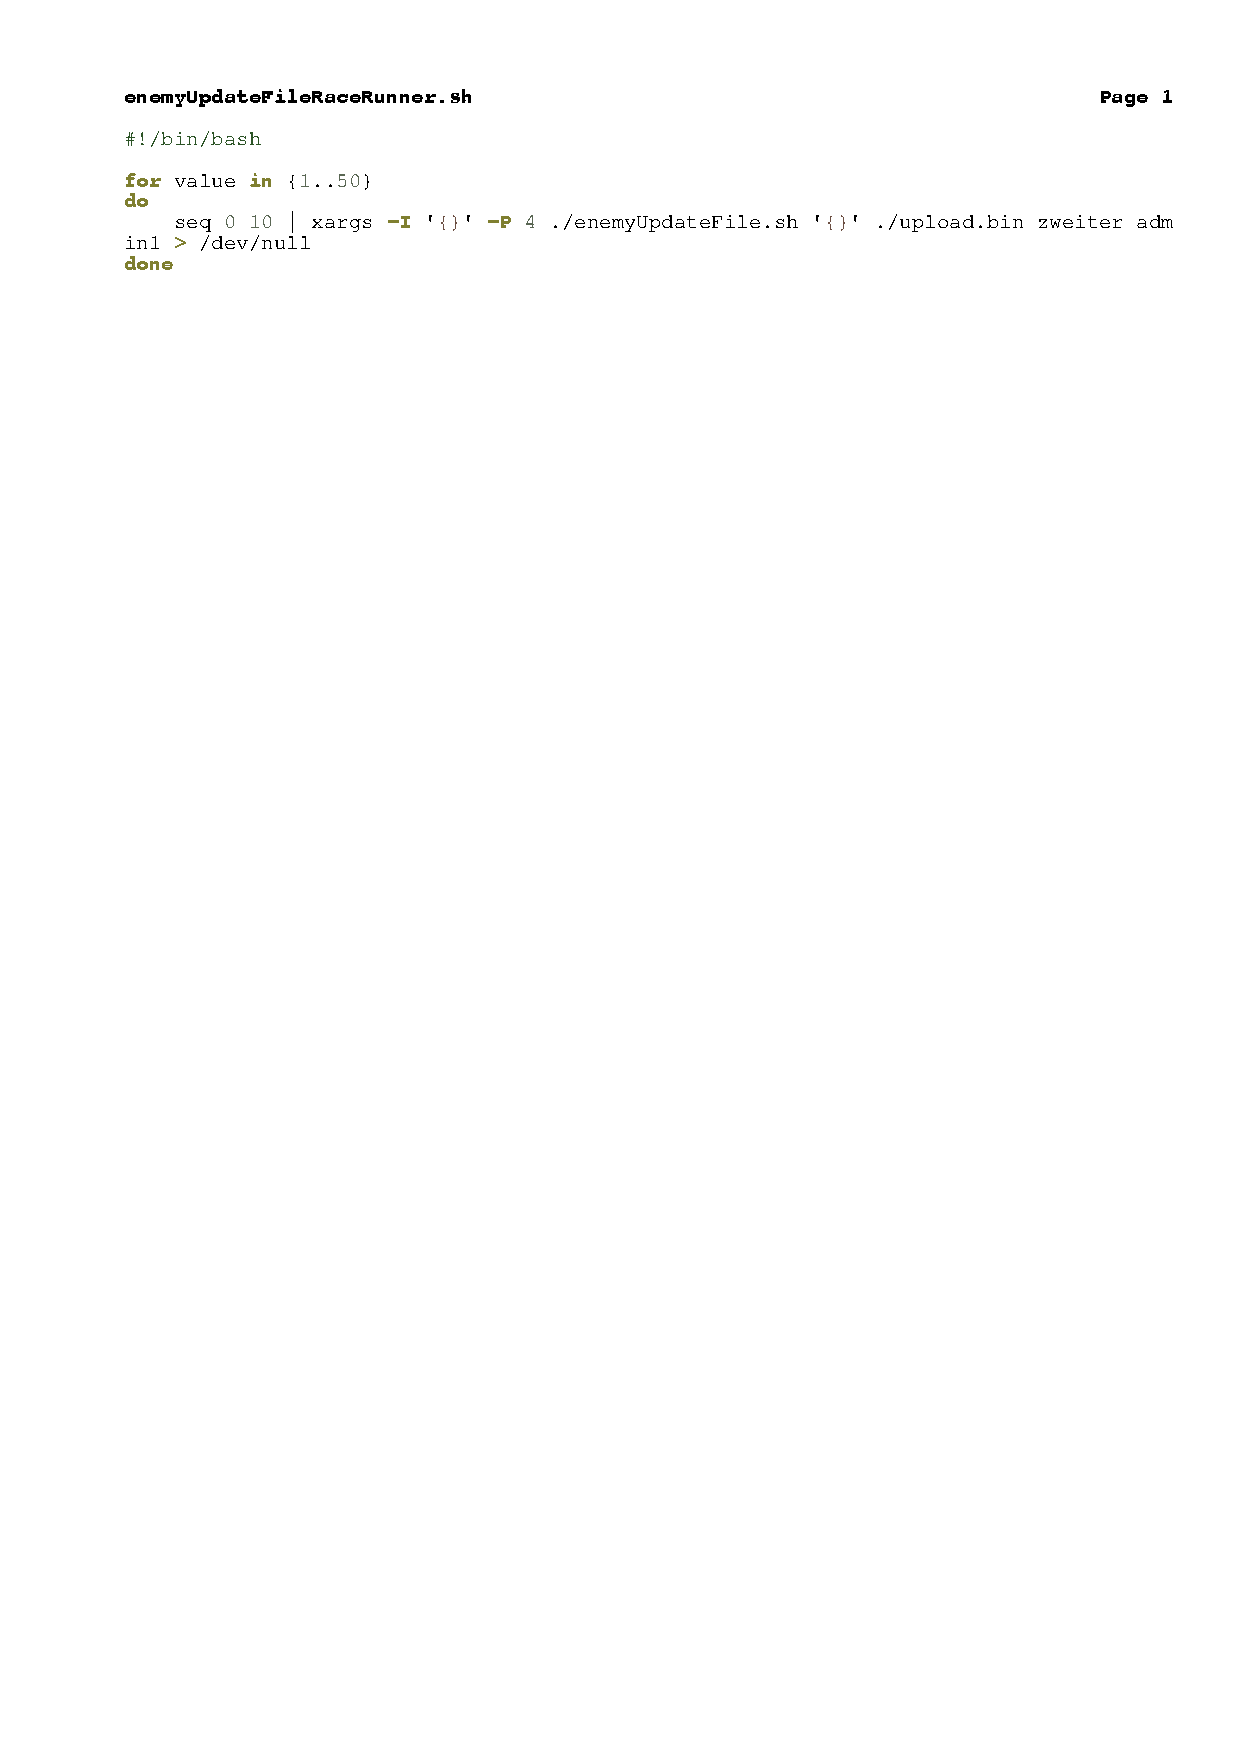
\includepdf{./resources/enemyQuotaRaceCondition_1.pdf}
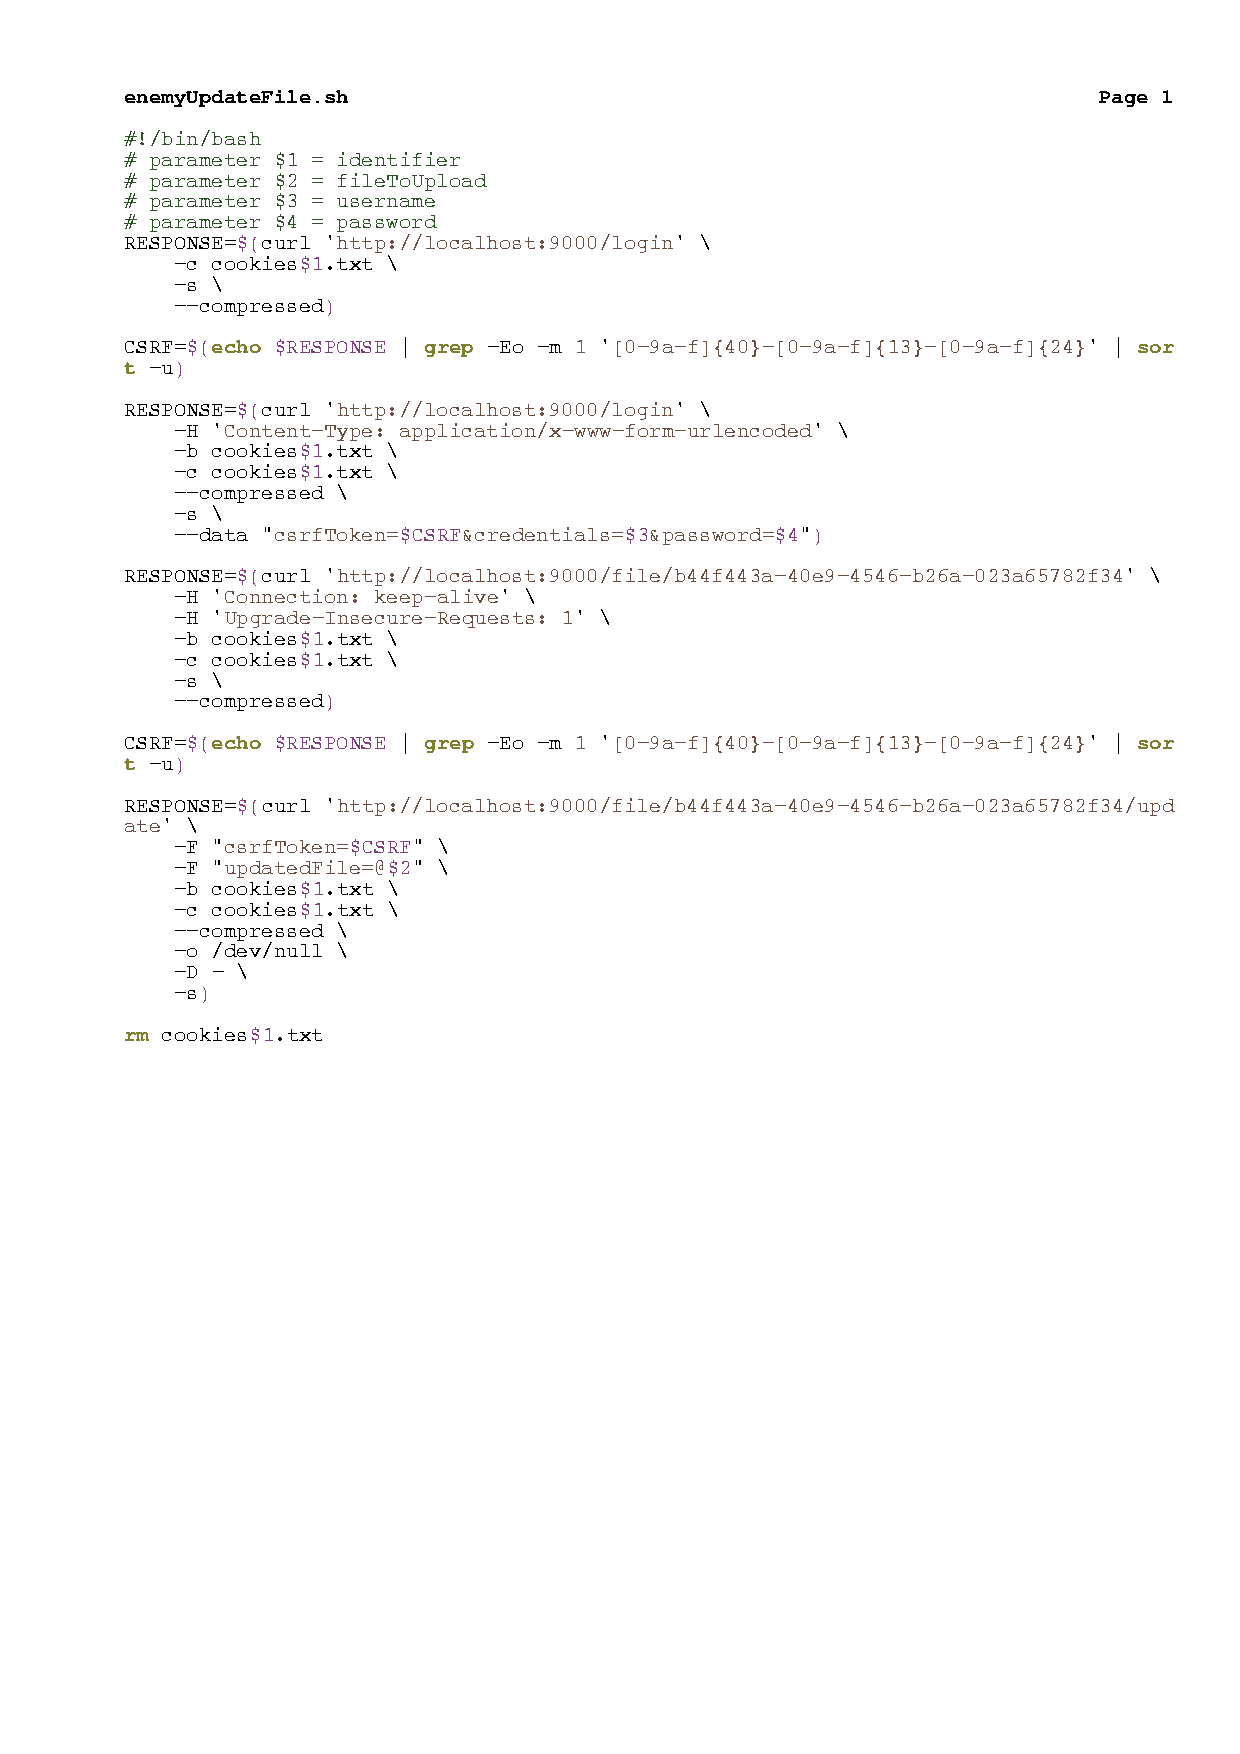
\includepdf{./resources/enemyQuotaRaceCondition_2.pdf}

\chapter{Fehler beim Anlegen eines neuen Nutzers in der bereitgestellten VM}

\begin{figure}[!htb]
  \centering
    \frame{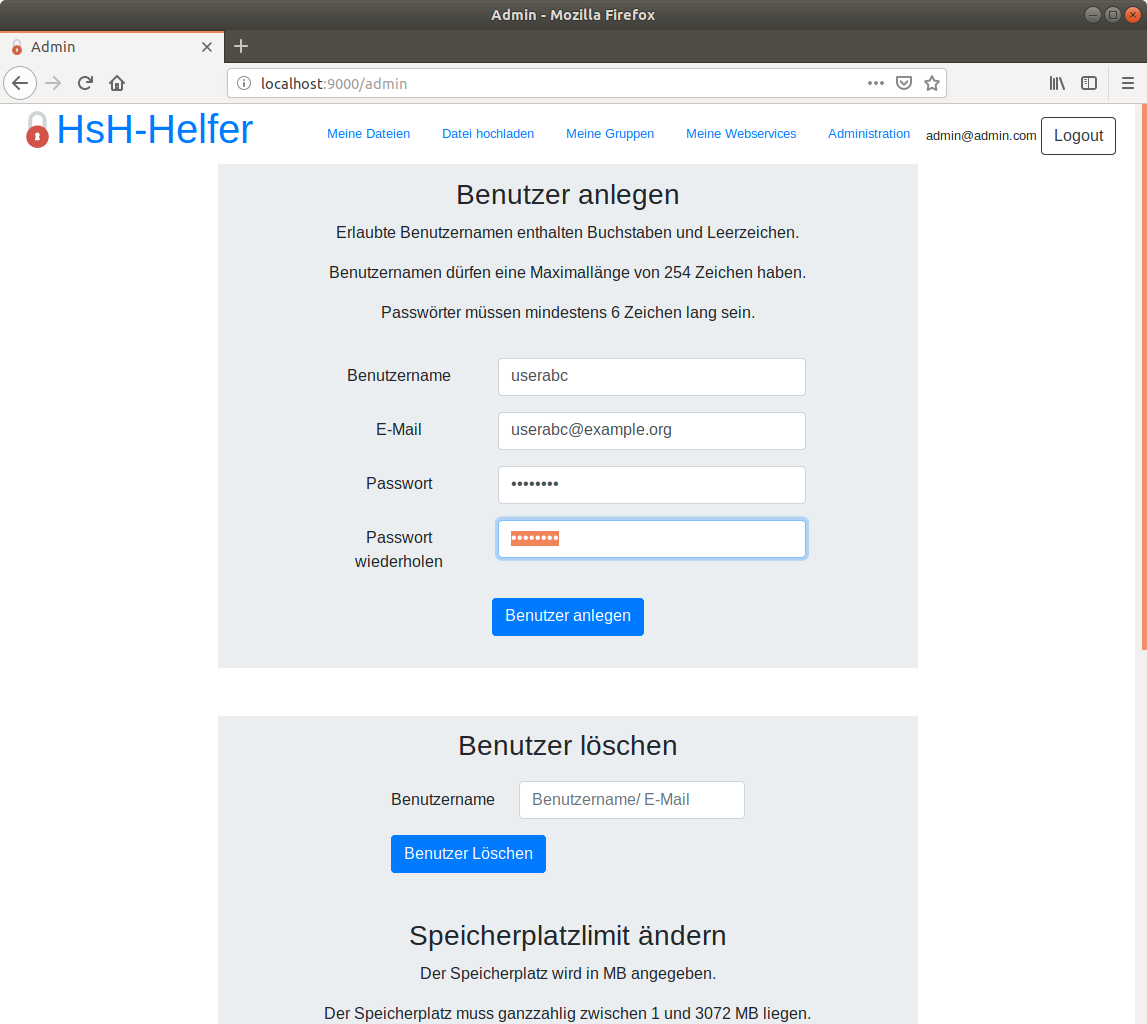
\includegraphics[width=0.8\paperwidth]{resources/createuser_fail_1.png}}
    \label{createuser_fail_1}
    \caption{Anlegen eines Nutzers in der bereitgestellten VM: Verwendete Daten}
\end{figure}

\begin{figure}[!htb]
  \centering
    \frame{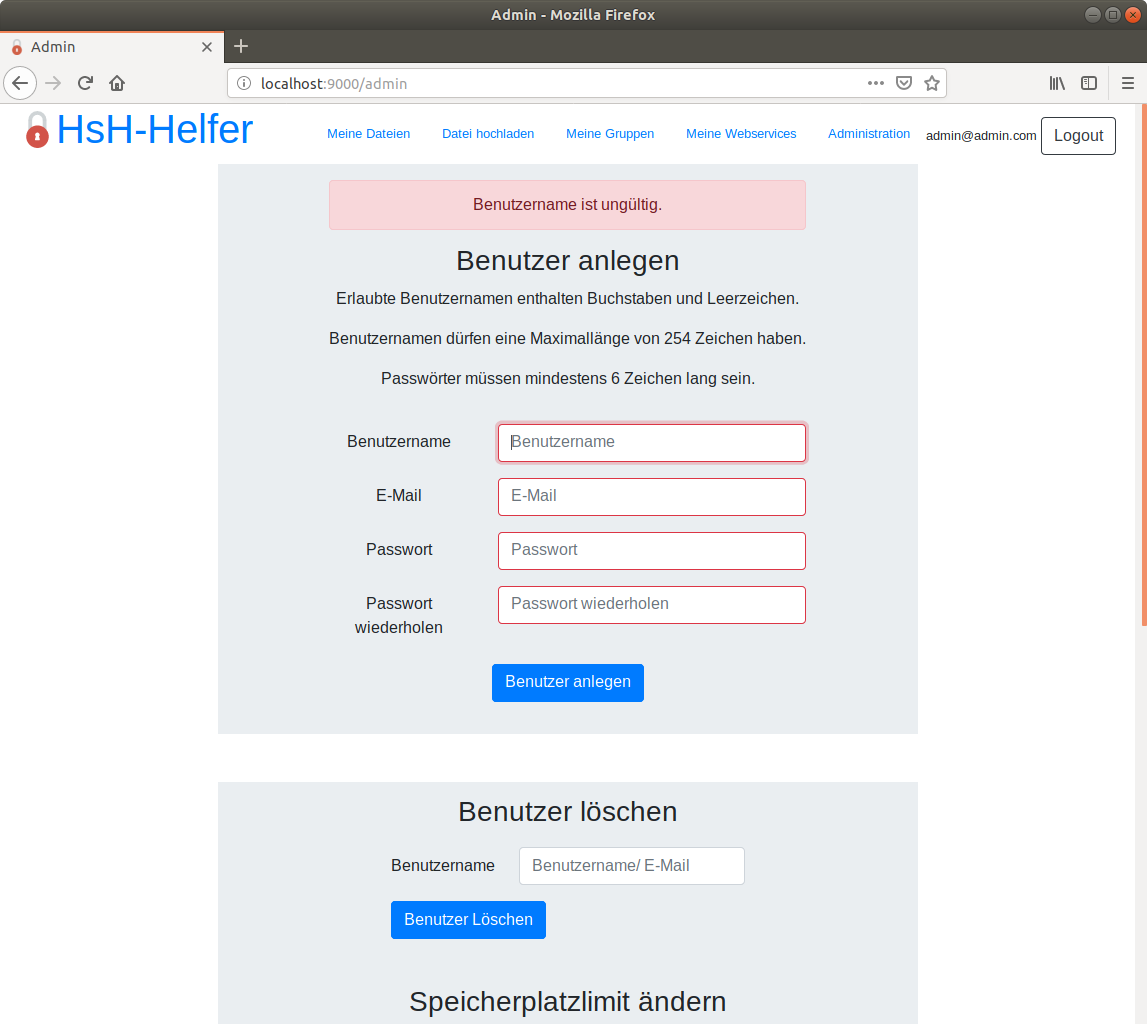
\includegraphics[width=0.8\paperwidth]{resources/createuser_fail_2.png}}
    \label{createuser_fail_2}
    \caption{Anlegen eines Nutzers in der bereitgestellten VM: Daraus resultierender Fehler}
\end{figure}

\chapter{Fehler beim Hochladen einer neuen Datei in der bereitgestellten VM}

\begin{figure}[!htb]
  \centering
    \frame{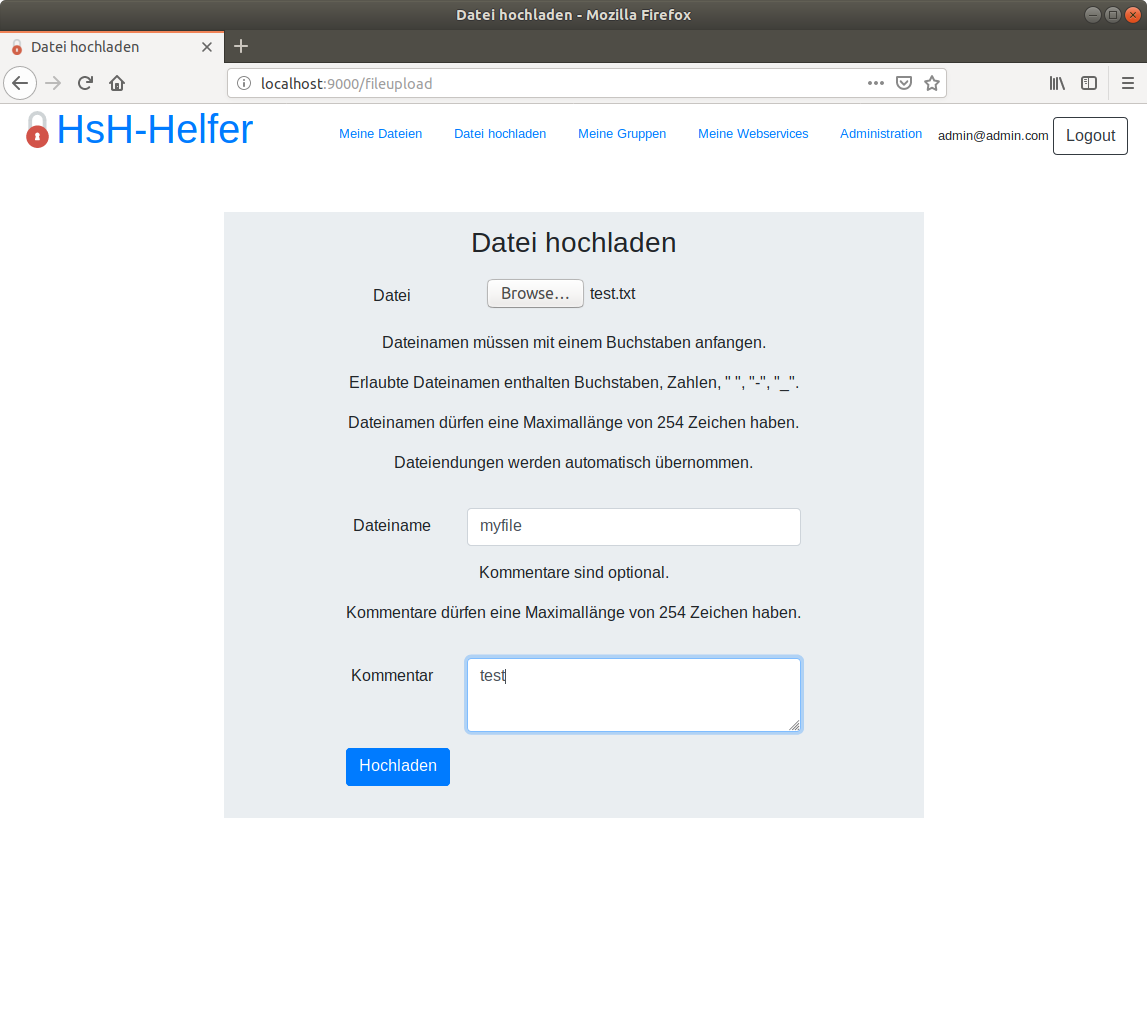
\includegraphics[width=0.8\paperwidth]{resources/upload_fail_1.png}}
    \label{upload_fail_2}
    \caption{Hochladen einer neuen Datei in der bereitgestellten VM: Verwendete Daten}
  \end{figure}

\begin{figure}[!htb]
  \centering
    \frame{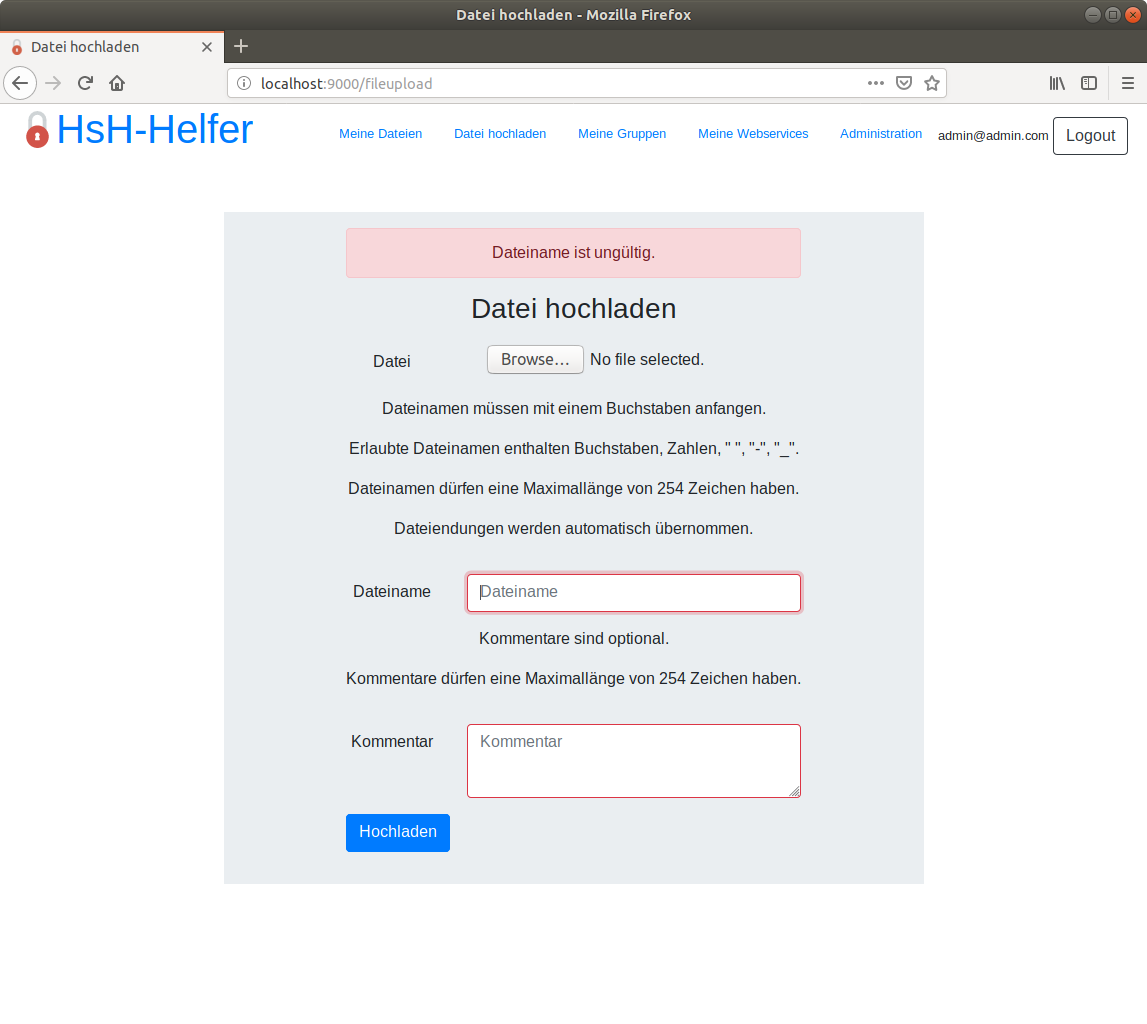
\includegraphics[width=0.8\paperwidth]{resources/upload_fail_2.png}}
    \label{upload_fail_1}
    \caption{Hochladen einer neuen Datei in der bereitgestellten VM: Daraus resultierender Fehler}
  \end{figure}

\chapter{Fileupload Racecondition Code}
 \label{fileuploadcode}
\begin{lstlisting}
// Check if user already uploaded a file with that name.
if (alreadyUploadedThatFilename(owner, filename)) {
    throw new DuplicateMemberException(
        String.format(Configuration.MESSAGE_FIELD_ALREADY_EXISTS, "Datei"));
}

// Get java file object.
java.io.File tempFile = fileMetadata.getFile();

// Read file size in MB.
final int fileSizeMb = bytesToMegaBytes(tempFile.length());

// Check if owner has sufficient quota to upload the file.
if (!owner.hasSufficientQuotaFor(fileSizeMb)) {
    throw new IndexOutOfBoundsException(
        Configuration.MESSAGE_EXCEED_QUOTA);
}

String fileExtension = FilenameUtils.getExtension(fileMetadata.getFilename());

// Create file metadata object.
model.File newFile = FileFactory.createFile(filename, fileExtension, comment,
    LocalDateTime.now(), tempFile.length(), owner);
\end{lstlisting}

\label{fileraceplugin}
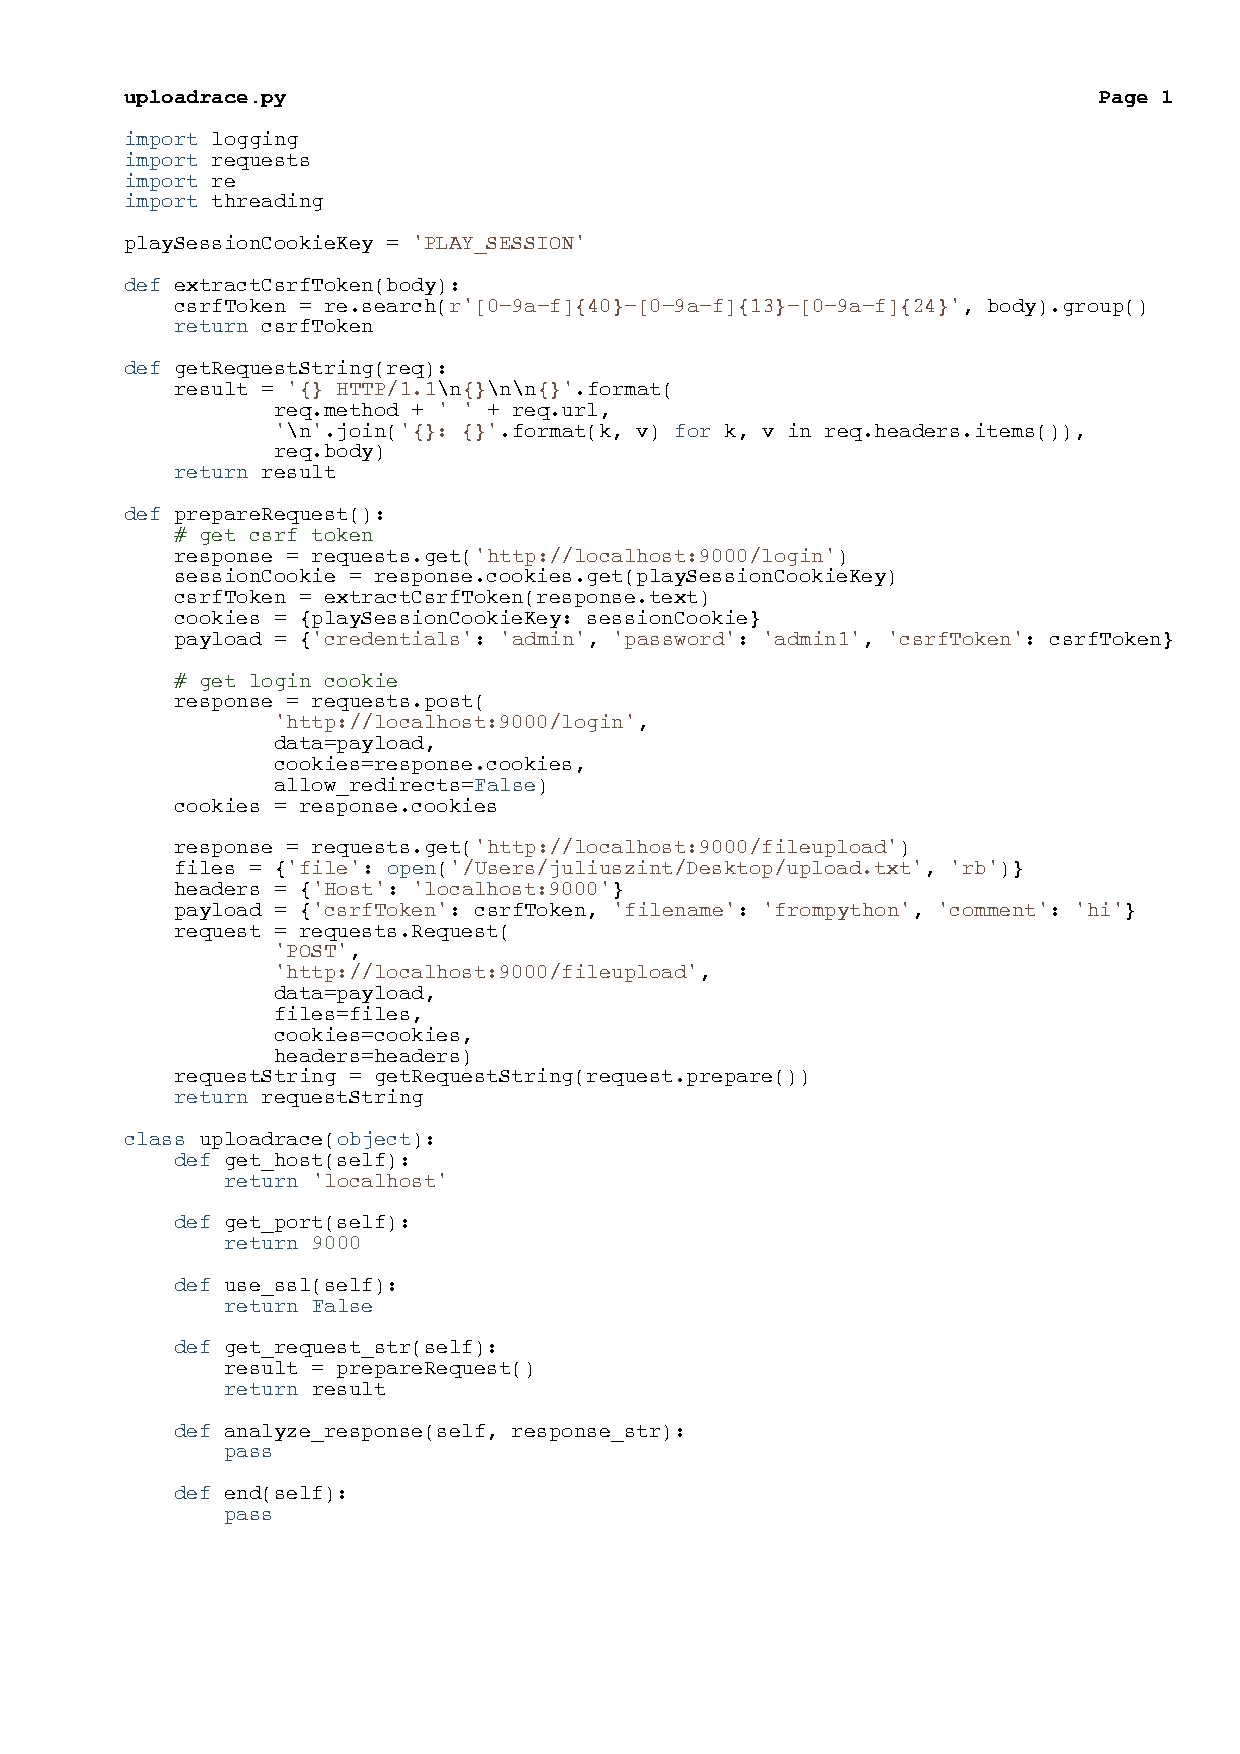
\includepdf{./resources/race_python.pdf}

\chapter{Code Beispiele}
\label{filepermissions}
\begin{lstlisting}
if ("read".equals(userPermission)) {
	for (String username : userList) {
		// Ignore Permission changes on owner
		// Should not occure, but better safe than sorry
		if (username.equals(file.getOwner())) {
		     continue;
		}
		User user = User.find.byName(username);
		grantReadAccess(user, file);
	}
}
\end{lstlisting}


\end{appendices}

\end{document}
